\section{Voltage Dividers}
\label{lab_voltage_dividers}

%\makelabheader %(Space for student name, etc., defined in master.tex)

\bigskip

\textit{For this lab and from now on, you'll want to make your circuits on your breadboards, using the internal power supplies on your PB-503 Proto-Boards.}

\begin{enumerate}[wide]

\item A voltage divider is a simple circuit made out of two resistors where the output voltage $V_{\rm out}$ is a fraction of the input voltage $V_{\rm in}$.  (Both $V_{\rm out}$ and $V_{\rm in}$ are measured with respect to ground, so $V_{\rm out}$ is actually the voltage across $R_2$.)  What is the ratio $V_{\rm out}/V_{\rm in}$ for the voltage divider shown below?  Make a prediction, then build it and test it.
 
\begin{center}

\includegraphics{voltage_dividers/voltage_divider.eps}
\end{center}

\item Design and build a voltage divider that will take an input of 5~V and give an output of 1~V.  (It's fine to combine multiple resistors from your kits in series or parallel to get whatever equivalent resistance you need.)  What is the power rating of your resistors?  Calculate whether they can handle the power demands of your circuit before turning it on. \label{part_five_to_one}

\item A trimpot (short for ``trimming potentiometer,'' which nobody actually says in real life) is a three-terminal variable resistor.  You can imagine a cylinder of an electrically resistive material, with fixed contacts on the top and bottom, and a third contact on the side that can slide up and down.  In your kit, the trimpots are small ($\sim 1$~cm) blue squares with white dials on them.  Use your DMM to measure the resistances between each pair of terminals of your trimpot marked ``5 0 2'' as you turn the dial.  Which of the terminals on your trimpots correspond to ``1'', ``2'', and ``3'' in the figure below?   

\begin{center}
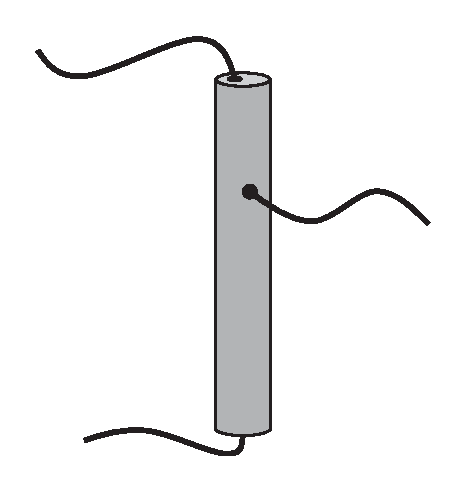
\includegraphics[height=0.9in]{voltage_dividers/trimpot_picture.eps}
\hspace{0.7in}
\raisebox{0.1in}{
\includegraphics{voltage_dividers/trimpot.eps}}
\end{center}

\item Bonus challenge: can you crack the secret code to decipher how the markings like ``5 0 2'' and ``1 0 3'' relate to the resistance of each trimpot in your kit?  

\item Use a single 5 k$\Omega$ trimpot to replace all of the resistors in the circuit you built in part \ref{part_five_to_one}.  Build it and test it.  What is the full range of output voltages you can get from it?  

\item Put some additional fixed resistors in series with a 1 k$\Omega$ trimpot to build a voltage divider that will use an input voltage of 5 volts and provide a variable output voltage that is adjustable between 1.0 and 2.0 volts.  (That is, those are the two output values when the trimpot is in its two most extreme positions.) \label{part_trimpot_exact}

\item Suppose you want to build a voltage divider with a $V_{\rm out}/V_{\rm in}$ ratio of exactly 0.50000.  If you use only a trimpot, then it can be very sensitive and difficult to set exactly.  On the other hand, if you use only fixed resistors, their values aren't guaranteed to be exact, and you may end up with a ratio of 0.510.  Use the same basic idea as in part~\ref{part_trimpot_exact} to design and build a voltage divider using two fixed 10 k$\Omega$ resistors and a trimpot, so that you can guarantee a ratio of exactly 0.500, provided the two fixed resistors are within their stated tolerances.  What value trimpot should you use?  Choose the smallest trimpot value possible for this.  (What's the downside if the trimpot value is too big?)  


\end{enumerate}

\begin{comment}
\textbf{Possible Exam Questions:}

\begin{itemize}
\item 	Design a voltage divider using a trimpot and two fixed resistors (100 k$\Omega$ and 200 k$\Omega$, both 1\% tolerance) that will guarantee that $V_{\rm out}/V_{\rm in} = 1/3$. What value trimpot is needed?
\end{itemize}
\end{comment}




